\documentclass[UTF8]{ctexart}
\usepackage{hyperref}
\usepackage{abstract}
\usepackage[margin=1in]{geometry}
\usepackage{graphicx}
\usepackage{gensymb}
\usepackage{float}
\usepackage{amsmath}
\CTEXsetup[name={第,章},number={\chinese{section}}]{section}
\begin{document}


\makeatletter
\newcommand\dlmu[2][4cm]{\hskip1pt\underline{\hb@xt@ #1{\hss#2\hss}}\hskip3pt}
\makeatother
\begin{center}
\zihao{3}
\begin{tabular}{rl}
\\
\\		 		   	   
&\textbf{设计实现有源巴特沃斯滤波器设计计算器的图形化界面} 	\\

\end{tabular}
\end{center}

\begin{center}
\zihao{3}
\begin{tabular}{rl}
\\
\\
\\
\\
\\	   		
\\
\\
\\
\\

&\makebox[4em][s]{班级}	\hspace{0.2cm}		\dlmu[5.5cm]{工物90}      \\
			   									 
&\makebox[4em][s]{学生姓名}	\hspace{0.2cm}	\dlmu[5.5cm]{张鸿琳}   \\
			   									 
&\makebox[4em][s]{学号}	\hspace{0.2cm}	\dlmu[5.5cm]{2019012137}   \\ 
			   									 
\end{tabular}
\end{center}

\newpage

\tableofcontents
\newpage

\section{巴特沃斯滤波器的简单介绍}
巴特沃斯滤波器的特点是通频带内的频率响应曲线最大限度平坦,没有起伏,而在阻频带则逐渐下降为零。 在振幅的对数对角频率的波特图上,从某一边界角频率开始,振幅随着角频率的增加而逐步减少,趋向负无穷大。其模满足:
\begin{equation}
|H(j\omega)|=\frac{1}{\sqrt{1+(\frac{\omega}{\omega_c})^{2N})}}
\end{equation}

由于该系统是实的且是稳定的,所以可以得到其传递函数为
\begin{equation}
\begin{aligned}
&H(s)=\frac{\omega_c^N}{\prod^{N/2}_{k=1}(s-p_k)(s-p_k^*)}=\frac{\omega_c^N}{\prod^{N/2}_{k=1}(s^2+2s\omega_c\sin(\frac{2k-1}{2N}\pi)+\omega_c^2)},N\ is\ even\\
&H(s)=\frac{\omega_c^N}{(s+\omega_c)\prod^{(N-1)/2}_{k=1}(s-p_k)(s-p_k^*)}=\frac{\omega_c^N}{(s+\omega_c)\prod^{(N-1)/2}_{k=1}(s^2+2s\omega_c\sin(\frac{2k-1}{2N}\pi)+\omega_c^2)},odd\\
\end{aligned}
\end{equation}

\section{利用巴特沃斯滤波器进行滤波器设计}
\subsection{Sallen-Key、MFB等设计滤波器常见结构}
滤波器设计时常常会用到Sallen-Key、MFB等结构,下面简单介绍设计\textbf{低通滤波器}(高通滤波器不再单独介绍)时用到的几个结构(下面的传递函数中的s与实际的$s'$的关系是$s'$=$s\omega_c$):
\subsubsection{普适Sallen-Key结构}
\begin{figure}[H]
\centering
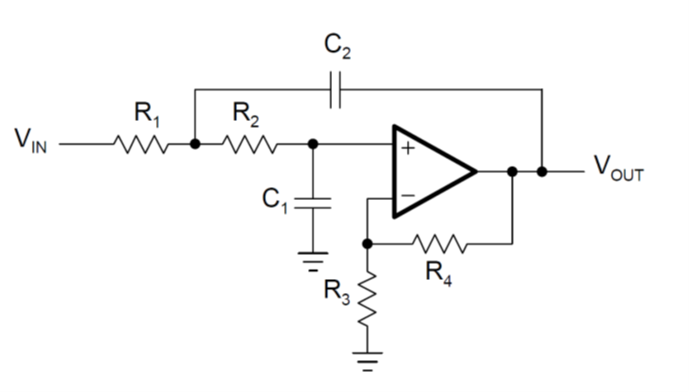
\includegraphics[width=0.5\textwidth]{1.png}
\caption{普适Sallen-Key结构电路图}
\end{figure}

其传递函数为:
\begin{equation}
A(s)=\frac{1+R_4/R_3}{1+\omega_c[C_1(R_1+R_2)-\frac{R_4}{R_3}R_1C_2]s+\omega_c^2R_1R_2C_1C_2s^2}
\end{equation}

为了计算便捷,本次设计没有采用该结构,而是采用了归一化的Sallen-Key结构,要素更少。
\subsubsection{归一化的Sallen-Key结构}
\begin{figure}[H]
\centering
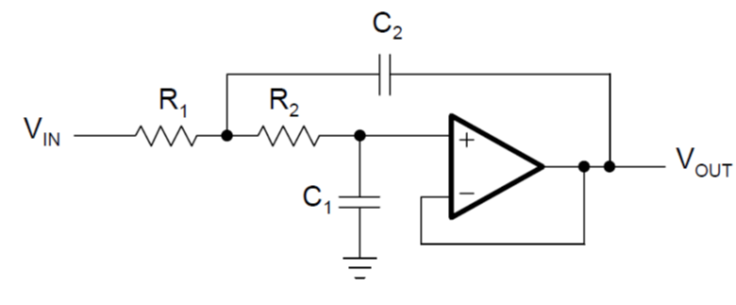
\includegraphics[width=0.5\textwidth]{2.png}
\caption{归一化的Sallen-Key结构电路图}
\end{figure}

其传递函数为:
\begin{equation}
A(s)=\frac{1}{1+\omega_cC_1(R_1+R_2)s+\omega_c^2R_1R_2C_1C_2s^2}
\end{equation}

\subsubsection{MFB结构}
\begin{figure}[H]
\centering
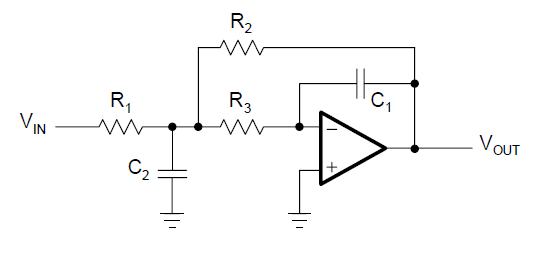
\includegraphics[width=0.5\textwidth]{3.png}
\caption{MFB结构电路图}
\end{figure}

其传递函数为:
\begin{equation}
A(s)=-\frac{\frac{R_2}{R_1}}{1+\omega_cC_1(R_2+R_3+\frac{R_2R_3}{R_1})s+\omega_c^2R_2R_3C_1C_2s^2}
\end{equation}

\subsubsection{一阶低通滤波器常用结构}
\begin{figure}[H]
\centering
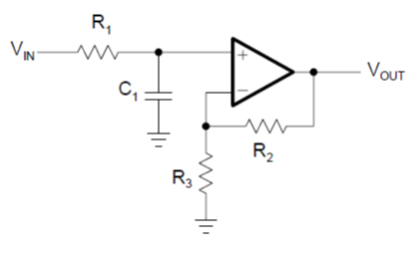
\includegraphics[width=0.5\textwidth]{4.png}
\caption{一阶同相低通滤波器电路图}
\end{figure}

其传递函数为:
\begin{equation}
A(s)=\frac{1+\frac{R_2}{R_3}}{1+\omega_cC_1R_1s}
\end{equation}

\begin{figure}[H]
\centering
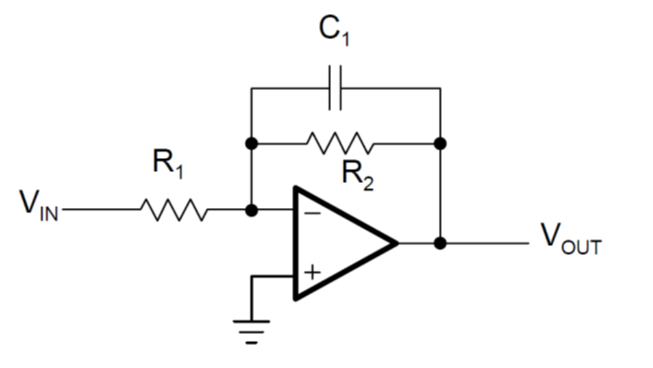
\includegraphics[width=0.5\textwidth]{5.png}
\caption{一阶反相低通滤波器电路图}
\end{figure}

其传递函数为:
\begin{equation}
A(s)=-\frac{\frac{R_2}{R_1}}{1+\omega_cC_1R_2s}
\end{equation}

\subsubsection{直流增益调节结构}
注意到上面的一些结构对直流增益范围有一定限制,所以需要直流增益调节结构,本次设计采用的结构如下(会引入反相):
\begin{figure}[H]
\centering
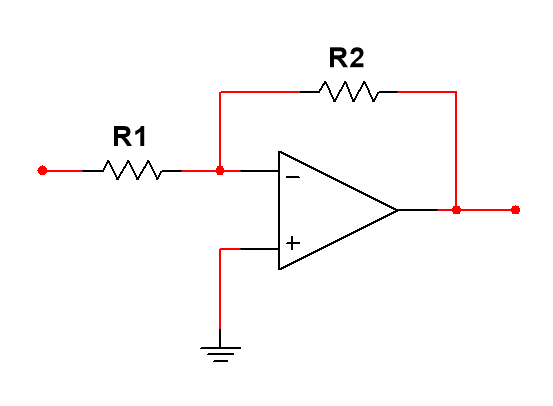
\includegraphics[width=0.5\textwidth]{6.png}
\caption{反相比例放大器电路图}
\end{figure}

调节$R_1$与$R_2$阻值大小可以对直流增益进行调节,但是会引入反相。

\subsection{基本步骤}
利用上面提到的几种结构以及巴特沃斯滤波器的性质,就可以进行基本的滤波器设计,基本步骤如下:

\begin{itemize}
\item 首先利用给定的通带频率和阻带频率,以及通带最大衰减和阻带最小衰减得到巴特沃斯滤波器的阶数
\item 再利用求得的滤波器阶数求得截止频率$\omega_c$
\item 根据阶数确定级联的结构,若阶数为奇数,则级联一个一阶滤波器和若干二阶滤波器(MFB结构或Sallen-Key结构),若阶数为偶数,则级联若干个二阶滤波器。最后再级联一个反相比例放大器用于调节直流增益
\item 根据相应阶数的巴特沃斯滤波器的各级系数以及截止频率,选定合理的滤波器元件参数
\end{itemize}
\section{利用matlab的GUI功能实现的有源巴特沃斯滤波器设计计算器的图形化界面}
\subsection{设计滤波器参数时的一些处理}
在确定滤波器元件参数时为了简化计算,减少变量,进行了一些处理:
\begin{itemize}
\item 在需要一阶低通滤波器的情况下,都采用了一阶同相滤波器结构,并令其中$R_2$与$R_3$的阻值相等,取$C_1$的值为10pF,调节$R_1$的值,使系统满足要求。
\item 考虑到实际的电容电阻值范围,对各个Sallen-Key结构的二阶低通滤波器都采用了归一后的较为简单的结构,并固定其中的$C_1$的值为1pF或10pF,同时令$R_1$与$R_2$的阻值相等,调节$C_2$的值使系统满足要求。(查到的资料中,一些是采用了令$C_1=C_2$的设计思路,而我采用令电阻阻值相等的方案是因为考虑到实际生产中电阻阻值的跨度大于电容值得跨度,所以这样或许有利于扩大该程序设计出的滤波器的合理的范围)
\item 对于MFB结构的二阶低通滤波器,都令$R_1=R_2=R_3$,并固定$C_1$的值为10pF或1pF,调节$C_2$的值使系统满足要求。
\item 由于上面的滤波器都通过增加等式关系的方法,限定了本身的直流增益,所以对所有的滤波器电路都增加了一个反相比例放大器,来调节直流增益,固定放大器中其中一个电阻的值,改变另一个电阻阻值来调节直流增益。(也可以采用将直流增益分摊给各级的方法,不过考虑到有些滤波器结构本身对直流增益范围有限制,所以这种方法相较之下更为简便,不过由于实际生产中电阻阻值大小的限制,这种方法可能会从一定程度上减小该程序设计出的滤波器的合理的范围)
\end{itemize}

由于没有足够的实际生产经验,所以这些处理可能并不十分合理,具体的讨论见“一些不足”。
\subsection{程序基本介绍与使用方法}
程序初始界面如下:
\begin{figure}[H]
\centering
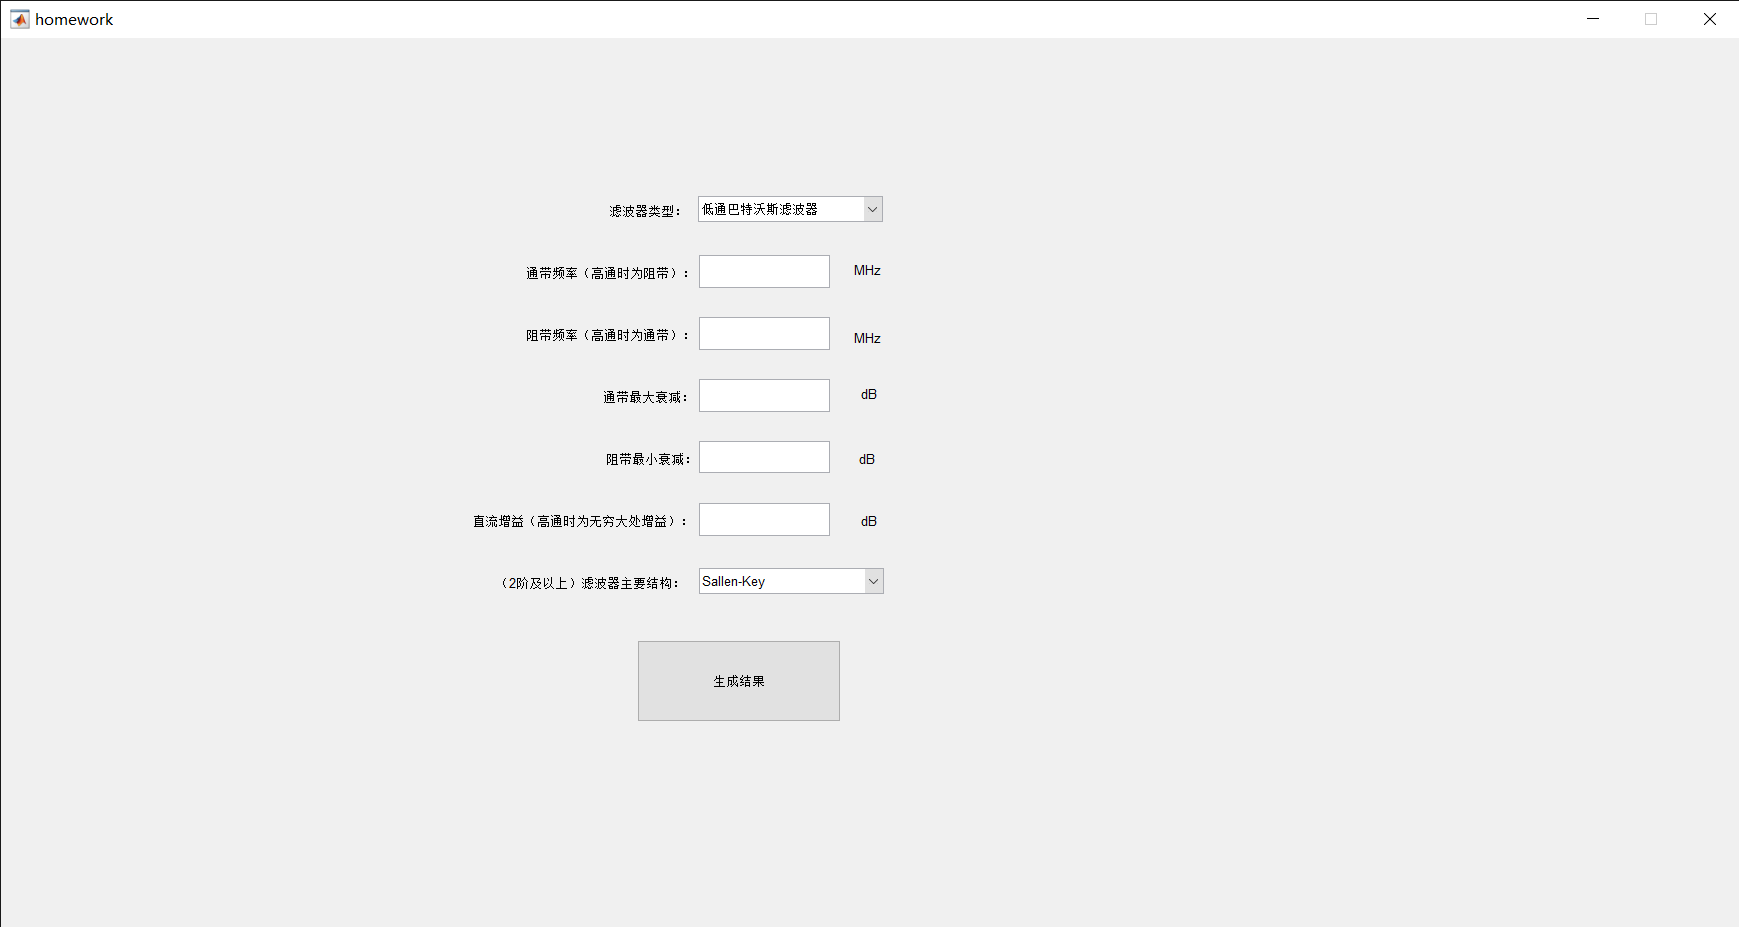
\includegraphics[width=\textwidth]{7.png}
\caption{程序初始界面}
\end{figure}

分别输入“通带频率”,“阻带频率”,“通带最大衰减”,“阻带最小衰减”,并选择滤波器类型和滤波器主要类型后点击按钮,如果数据有误,会报错提示重新输入,如果数据比较正常,且对应巴特沃斯滤波器阶数低于8,程序就会刷新界面,生成结果,如下图:
\begin{figure}[H]
\centering
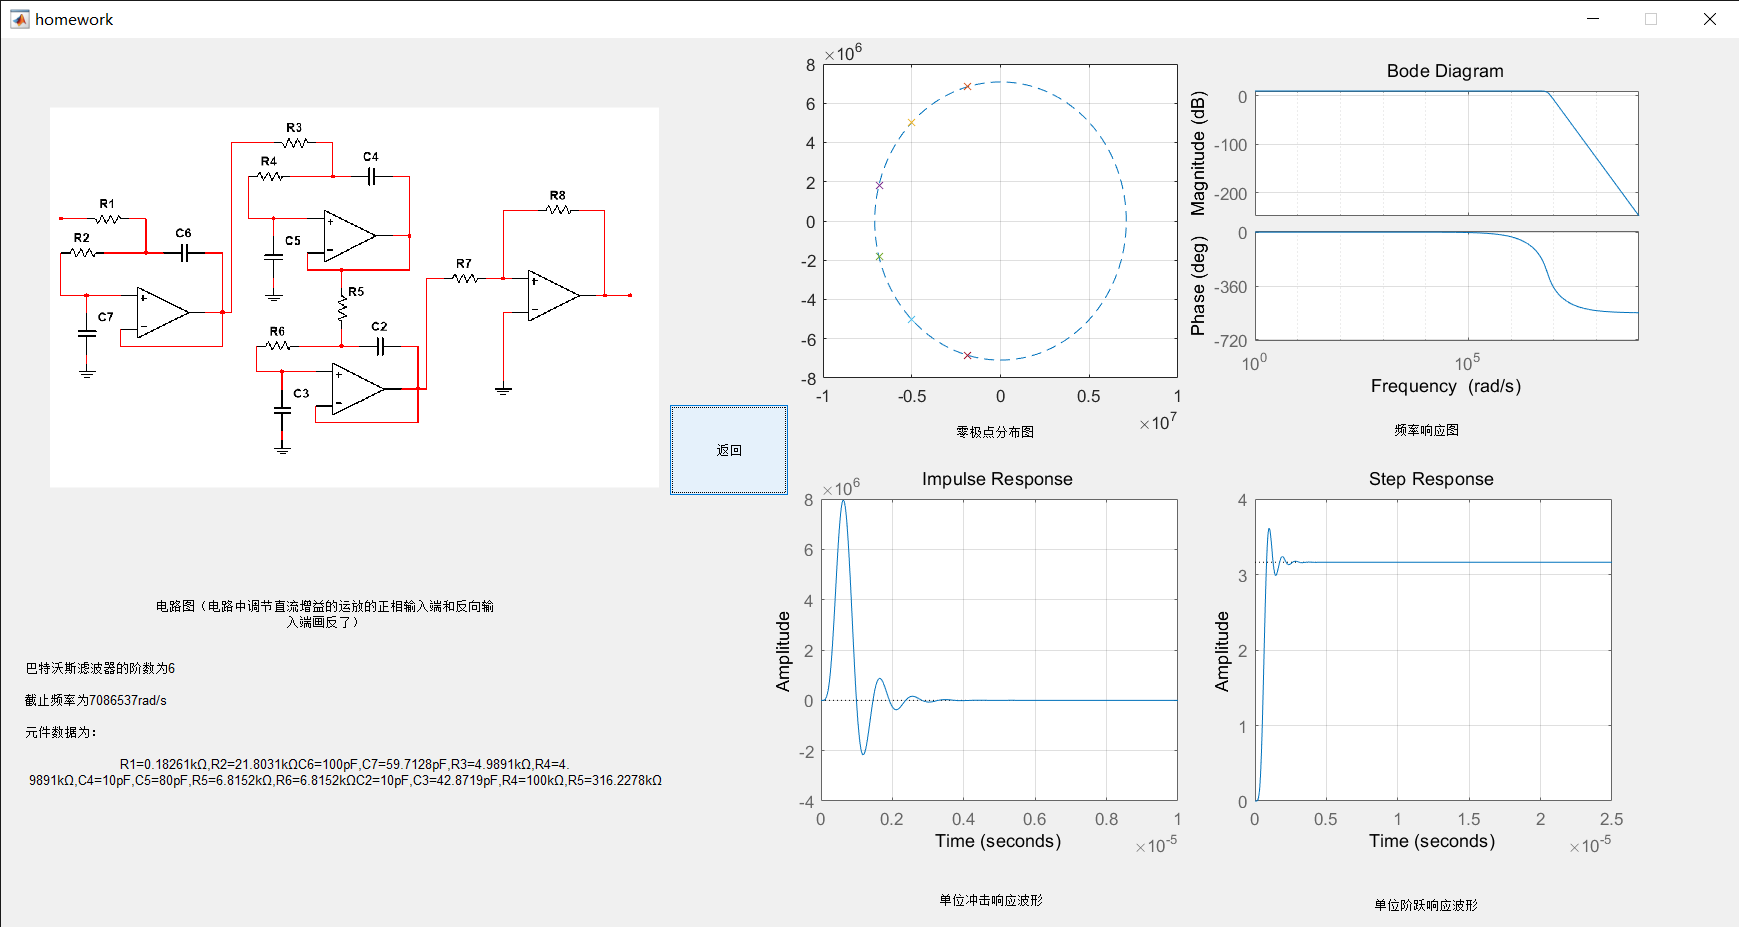
\includegraphics[width=\textwidth]{8.png}
\caption{输出结果界面}
\end{figure}

结果界面包含输入信息对应的巴特沃斯滤波器的零极点图、伯德图、单位冲激响应、单位阶跃响应、滤波器电路图,同时左下角会显示滤波器的一些基本数据(高通滤波器的元件参数来不及处理,左下角只会显示滤波器阶数和截止频率),点击“返回”按钮会返回初始界面,可重新处理新的数据。

程序的源代码见压缩包。
\subsection{一些不足}
由于个人经验不足,时间仓促,该程序存在一些不足:
\begin{itemize}
\item 没有完全完成高通滤波器的元件参数的计算,只完成了高通滤波器电路图的输出
\item 对于输入的限制与纠错较少,可能存在一些不合理的输入导致生成不合理的输出
\item 元件参数的展示比较粗糙,实际上,如果能以表格形式展示会更清晰
\item 输出图像的信息比较模糊,坐标不够完善,很难准确体现出比较精准的数据
\item 上面采用的为了简化计算而进行的处理可能并不能很好地与现实中的生产条件对应,调节直流增益的方法比较笨拙,所以可能还需要调整,而且一些处理方法不够灵活,导致限制较多,能够自由调节的元件参数值较少
\item 电路图不够精细和整洁(个别运放的同相输入端和反向输入端画反了)
\item 没有处理好反相给传输函数带来负号的问题
\item 一些图像限制了坐标轴范围,可能导致图像不完整

\end{itemize}

\begin{thebibliography}{123456} 
\bibitem{ref1} 康绍耕.《MATLAB GUI编程显示载入.JPG图片》.
\bibitem{ref2} iLoveMatlab论坛.《matlab GUI 新手入门——最基本的几个概念》.
\bibitem{ref3} Texas Instruments.《Active Filter Design Techniques》.
\end{thebibliography}


\end{document}
